\documentclass[8pt, oneside]{article}   	
\usepackage[top=1in, bottom=1in, left=1.5in, right=1.5in]{geometry} 		
\geometry{letterpaper}                   		

\usepackage{hyperref}
\usepackage{graphicx}												
\usepackage{amssymb}
\usepackage{amsmath}
\usepackage{array,multirow,graphicx}
\usepackage{float}
\usepackage{rotating}
\usepackage{adjustbox}
\usepackage{subcaption}
\usepackage{Times}
\usepackage[margin=1cm]{caption}

\title{Improving BISP household targeting through estimation of poverty from satellites, Facebook advertising data and Open Street Maps}
%\author{Rob Marty and Alice Duhaut}

\begin{document}

\maketitle


\section*{Purpose}

While the National Socio-Economic Registry (NSER) gives a precise estimate of poverty using door-to-door questionnaires, it is a costly survey and can only be fielded infrequently. In this short work, we show how a simple machine learning algorithm applied to open source daytime and nighttime satellite imagery, Facebook advertising data and Open Street Map (OSM) data can be used to help BISP predict poverty and improve its targeting mechanisms. To demonstrate the validity of the approach, the following work uses Oxford Policy Management (OPM) household surveys to train the algorithm. We find that the algorithm correctly identifies 68.23\% of poor households in 2014. This information can be used to detect errors of inclusion and exclusion in the NSER, and better identify poor households especially between the different rounds of NSER updates, and create more reliable poverty indicators in neighbourhoods with low survey response rates.

\section*{Methods}

While daytime and nighttime satellite imagery is increasingly available both at the global scale and with refined granularity, these data are often inherently unstructured and pose challenges in processing and manual analysis. For example, while some of these characteristics are easily interpretable - nighttime lights corresponding to the public and private light fixtures in a given neighborhood, green cover corresponding to garden and parks - some are less obvious - blue and red lights reflected have no obvious relationship to household characteristics. In response to these challenges, we employ deep learn methods, a convolutional neural network (CNN) in particular, to extract features from these satellite imagery to be used on our poverty estimation model. 

\subsection*{Transfer Learning}
Applications of deep learning techniques to image data are now common in computer vision, especially in performing tasks like object detection or object classification. These techniques, however, are most effective with ample labeled training data. In our task, while a CNN could be trained to directly estimate poverty from satellite imagery, limited training data on poverty outcomes makes this application challenging. With only slightly over 3000 data points for poverty in Pakistan for the year 2014, we cannot directly train a large CNN model to estimate poverty from satellite images. Instead, we turn to a transfer learning approach. Given a suggested correlation between nighttime light radiance and economic well-being, we choose to use nighttime lights as a proxy in our larger poverty estimate task. In this approach, we train a fully-convolutional CNN model to estimate nighttime light radiance from daytime light satellite images. By solving this proxy task, the model learns how to extract features that are also useful for the poverty estimation.

\subsection*{Image Feature Extraction}
In the first step of the transfer learning approach, we divide Pakistan into 200-meter grids called tiles. We then train a 5-layer CNN Sequential model to estimate nighttime light radiance corresponding to a given tile in daytime satellite images. We transform nighttime light radiance using the natural logarithm to lessen the presence of skewness and then divide into five ordinal classes, representing low to high radiance, using K-means clustering. These class distinctions were determined by observing the spread of nighttime light radiance in our training set, which includes over one million nighttime light radiance data points for areas in Pakistan. 
\par
The model is trained using early stopping of epoch trials to reduce overfitting and five-fold cross-validation. We train our CNN on all seven available raster bands for daytime satellite data, allowing for a data representation that is richer than those yielded from processing BGR images alone. After training the CNN model to predict nighttime light radiance, we use this learned model as a feature extractor for daytime satellite images by discarding the last layer of the CNN model, which serves as the nighttime light classification layer. 

\section*{Poverty Estimation}

\subsection*{Image Feature Extraction and Dimensionality Reduction}
In predicting household poverty, we spatially link each household to the daytime light satellite image tile in which it is located. We then use our trained CNN to extract features. The CNN extracts 100-dimensional feature vectors from daytime light satellite images. We find that using principal component analysis (PCA) to reduce the dimension retains most of the pertinent feature information. Reducing to the first 10 principal components retains over 94\% of explained variance. This dimensionality reduction provides two main benefits: it reduces computational costs and serves as a second guard against overfitting by allowing a model of reduced complexity represent the the underlying relationships.

\subsection*{Additional Features}
In addition to geospatial features, the method also extracts the number of monthly and daily active Facebook users within the 1 square km circle. This approach relies on Facebook's marketing platform, which allows determining the number of Facebook users of different characteristics. As of now, we extract the number of male and female active users; however, many other subsets are possible that likely correlate with poverty levels such as the number of users with a select educational background and the type of phone used to connect to facebook (e.g., high end or cheap phone). 
\par
In addtion, the algorithm extracts the distance of a household to different road types using Open Street Map (OSM) data; for example, we calculate the distance of households to the nearest road and nearest type of road, including the nearest trunk road and residential road. See appendix A for further description of the OPM data and appendix B for further description of the data sources used for poverty estimation.

\subsection*{Handling of Imbalanced Data}
Our available data consisted of 3259 households. Of these 3259 households, 1022 were considered poor and 2237 were considered not poor. That is, poor households amounted to less than one-third of total households and roughly 46\% of not poor households. In a binary classification task, this level of imbalance can critically hinder performance. In response to this, we randomly over-sample the minority class, poor households, until poor households constitute 65\% of not poor households. We choose not to simply create equal class sizes for two reasons. Under-sampling the majority class, not poor households, discards valuable training data and oversampling the minority class to meet the same frequency as the majority class disregards the a major relationship - poor households are not as prevalent as not poor households. To retain the information in this relationship, we choose to oversample with this strategy, ultimately only increasing the total share of poor households by roughly 8\%.

\subsection*{Model and Feature Selection}
We select our best model for poverty estimation by performing a hyper-parameter grid search on eight different classification models with a 80-20 train-test split. In performing the grid search, we also define five different feature groups on which to train our models. The feature groups tested are the following: numeric representations daytime light and nighttime light radiance, OSM and Facebook data, features extracted using our CNN, OSM and Facebook data along with features extracted using our CNN, and all aforementioned features.
\par
We realize that one potential application of poverty classification is to identify households for assistance programs or other such programs in which poor households would be the targeted beneficiaries. Given this potential application, our foremost consideration is guarding against overlooking or missing poor households in our classification so long as classification for our majority class is sufficiently performing. To achieve this, we define a simple metric for evaluating models in our grid search.

\begin{equation*}
  score = max(recall_{not poor},  recall _{poor}) - \lvert recall_{not poor} - recall _{poor} \rvert
\end{equation*}
\par
The resulting best model was an AdaBoost Classifier model with five estimators and a Decision Tree Classifier of maximum depth ten as its base estimator trained on OSM and Facebook data along with features extracted using our CNN. On testing data, the model performed at 70.0\% accuracy, 58.5\% precision, 68.2\% recall for poor households, and 71.0\% recall for not poor households. The feature group associated with our best model suggests the benefits of extracting features from satellite images using a trained CNN, which, unlike their numerical representations, can contain underlying geospatial properties of the images themselves.

\section*{Results}
Our transfer learning model is strongly predictive binary poverty as measured at the household level in 2014 Pakistan. In generating predictions for all 2014 households, our model performed at 90.7\% accuracy, 83.4\% precision, 88.0\% recall for poor households, and 92.0\% recall for not poor households.
\par
Note that false negative results are both low at 3.48\% and the least likely outcome, minimizing the likelihood of overlooking poor households (see Figure 1(a)). Nine of the ten most salient features in our model are features gathered from OSM (see Figure 1(b)). While this suggests that distance from different roads is a key contributing relationship to the poverty states of households, the inclusion of extracted features in the feature group selection associated with our best model suggests a nontrivial added predictive power in including features with maintained underlying geospatial information.
\par
The data used here is both entirely publicly available and passively collected. The ability to harness their predictive power and produce reasonable estimates of poverty can improve or validate poverty estimates collected through more traditional means. Additionally, employment of simple machine learning algorithms to extract meaningful information from these data, can also provide a functional yet cost-effective framework for testing preliminary research hypotheses.
\par

\begin{figure}[ht]
\begin{subfigure}{.45\textwidth}
  \centering
  % include first image
  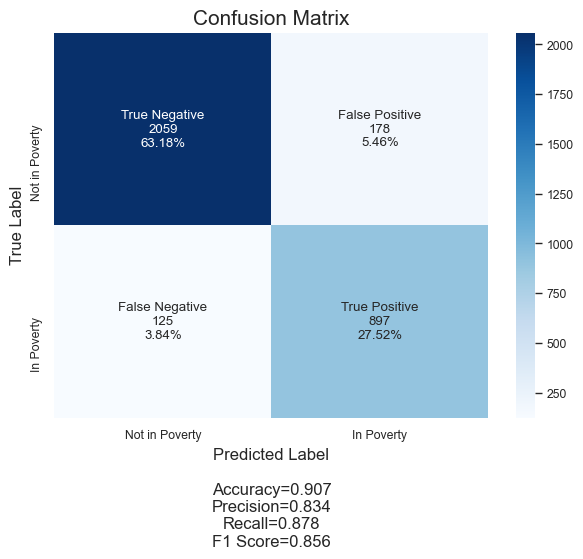
\includegraphics[width=1\textwidth]{Figures/confusion_matrix.png}   
  \caption{Poverty Estimation Outcomes}
  \label{fig:sub-first}
\end{subfigure}
\begin{subfigure}{.55\textwidth}
  \centering
  % include second image
  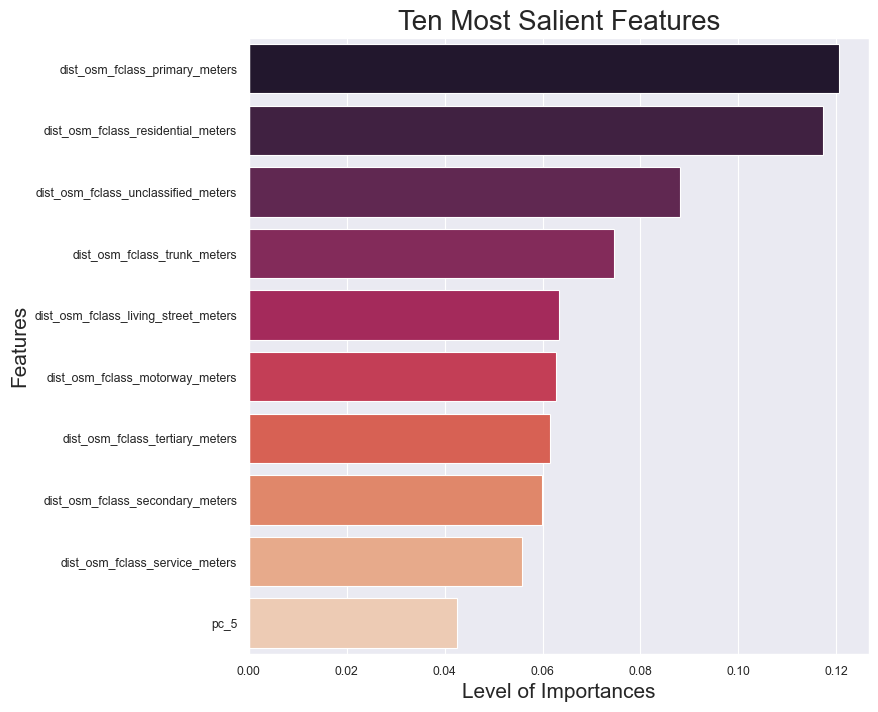
\includegraphics[width=1\textwidth]{Figures/feature_importances.png}   
  \caption{Feature Importances}
  \label{fig:sub-second}
\end{subfigure}
 \caption{Key Results}     
\label{fig:pscore_change_hist}
\end{figure}

\begin{figure}[H]
\label{fig:map}
\centering
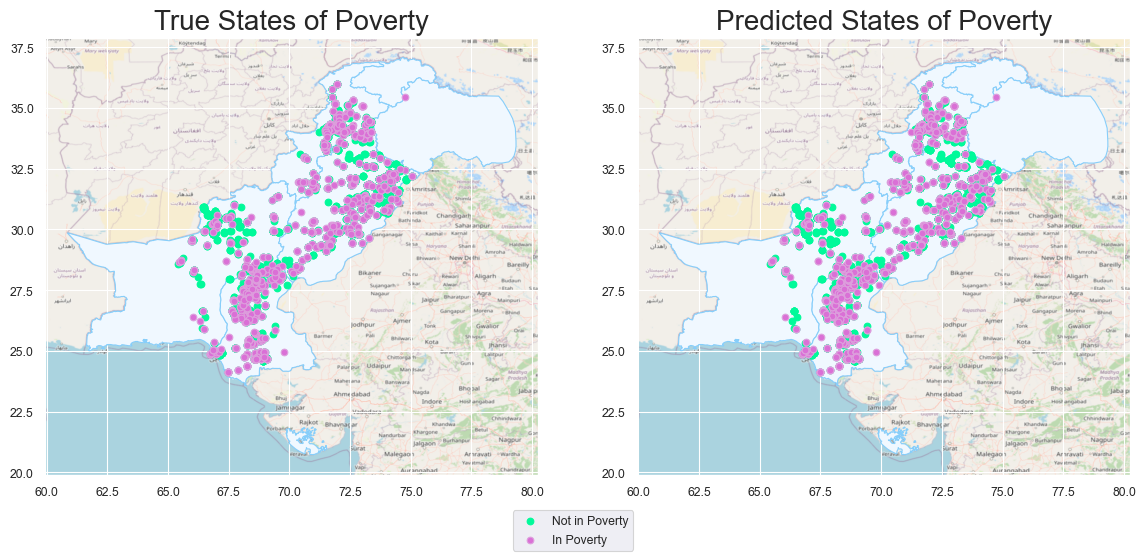
\includegraphics[width=1\textwidth]{Figures/map.png}
\caption{True vs. Predicted Labels}
\end{figure}

\newpage

\section*{Data limitations }

This approach performs best when it is fed with the most precise and granular data, and a larger sample of households. In addition, the algorithm will work best when values of poverty are representative of a spatial area. A limitation of the current approach is that the OPM survey data we are using is only representative at the national level, making it difficult to make predictions at a more local level, e.g. union councils.

\section*{Next Steps for Analysis}

The current approach shows that nontraditional data sources, including satellite and Facebook data, achieve a reasonable level of accuracy in predicting local levels of poverty. If given access to the more comprehensive NSER database, we plan to refine the analysis in five ways: 
\begin{enumerate}
\item Use more complex algorithms that require larger amounts of data
\item Explore how well the algorithm can predict the distribution of poverty levels as opposed to just a binary poverty indicator
\item Explore how well the algorithm can predict changes in poverty, as opposed to just levels
\item Explore which components of poverty the algorithm can best explain (e.g., overall poverty score, specific combination of assets, etc)  
\item Use additional methods and datasets to determine which factors the algorithm relies on in generating income/poverty estimates (e.g., nighttime lights, vegetation, presence of streets, orderliness of streets, etc)
\end{enumerate}
 If granted access to data representative at the Tehsils or Union Council levels, the team will be able to advance the algorithm to achieve higher accuracy and reliably predict poverty at lower administrative levels.

\newpage
\appendix
\section*{Appendix}

\section{OPM Data}

We rely on four rounds of survey data from the Benazir Income Support Project (BISP) for poverty data, surveyed in 2011, 2013, 2014 and 2016. Roughly 8,000-9,000 households were surveyed each year across Pakistan; however, geographic coordinates were only recorded in 2011 and 2013 and within these years only about half the households had coordinates recorded (see \autoref{tab:bisp_sum_stat}). For households that were resurveyed in 2014 and 2016 we rely on the geographic coordinates of the households in 2011 and 2013. Average poverty scores and the proportion of households considered poor are roughly the same between the full sample of households and the sample with coordinates for all years except 2016. 
\par
\autoref{fig:pscore_change_hist} shows changines in the number of household poverty over time. \autoref{fig:pscore_change_hist}a shows notable churning of households moving above and below BISP's threshold for household poverty, and \autoref{fig:pscore_change_hist}b shows notable changes in the poverty scores between 2011 and 2014. Moving forward, we are exploring whether nontraditional data can capture these changes in poverty. However, additional data---such as the NSER---will likely be required to train an algorithm able to capture changes in poverty.  

\begin{table}[H]
\caption{BISP Summary Statistics}
\label{tab:bisp_sum_stat}
\centering
\begin{tabular}{cc|ccc|ccc} 
\hline 
       &      & \multicolumn{3}{c|}{Full Sample} & \multicolumn{3}{c}{Sample with Coordinates} \\ 
\hline 
Survey & Year & Number of  & Average       & Proportion & Number of  & Average       & Proportion \\ 
Round  &      & Households & Poverty Score & Poor       & Households & Poverty Score & Poor \\ 
\hline 
1 & 2011 & 8675 & 18.44 & 0.48 & 4793 & 18.71 & 0.47  \\ 
2 & 2013 & 8221 & 22 & 0.35 & 4368 & 22.63 & 0.33  \\ 
3 & 2014 & 7759 & 22.96 & 0.31 & 3273 & 22.91 & 0.31  \\ 
4 & 2016 & 9139 & 23.4 & 0.28 & 1313 & 20.47 & 0.38  \\ 
\hline 
\end{tabular} 

\flushleft \footnotesize The full sample includes all households while the sample with coordinates only includes households with a geocode.
\end{table}

\begin{figure}[ht]
\begin{subfigure}{.45\textwidth}
  \centering
  % include first image
  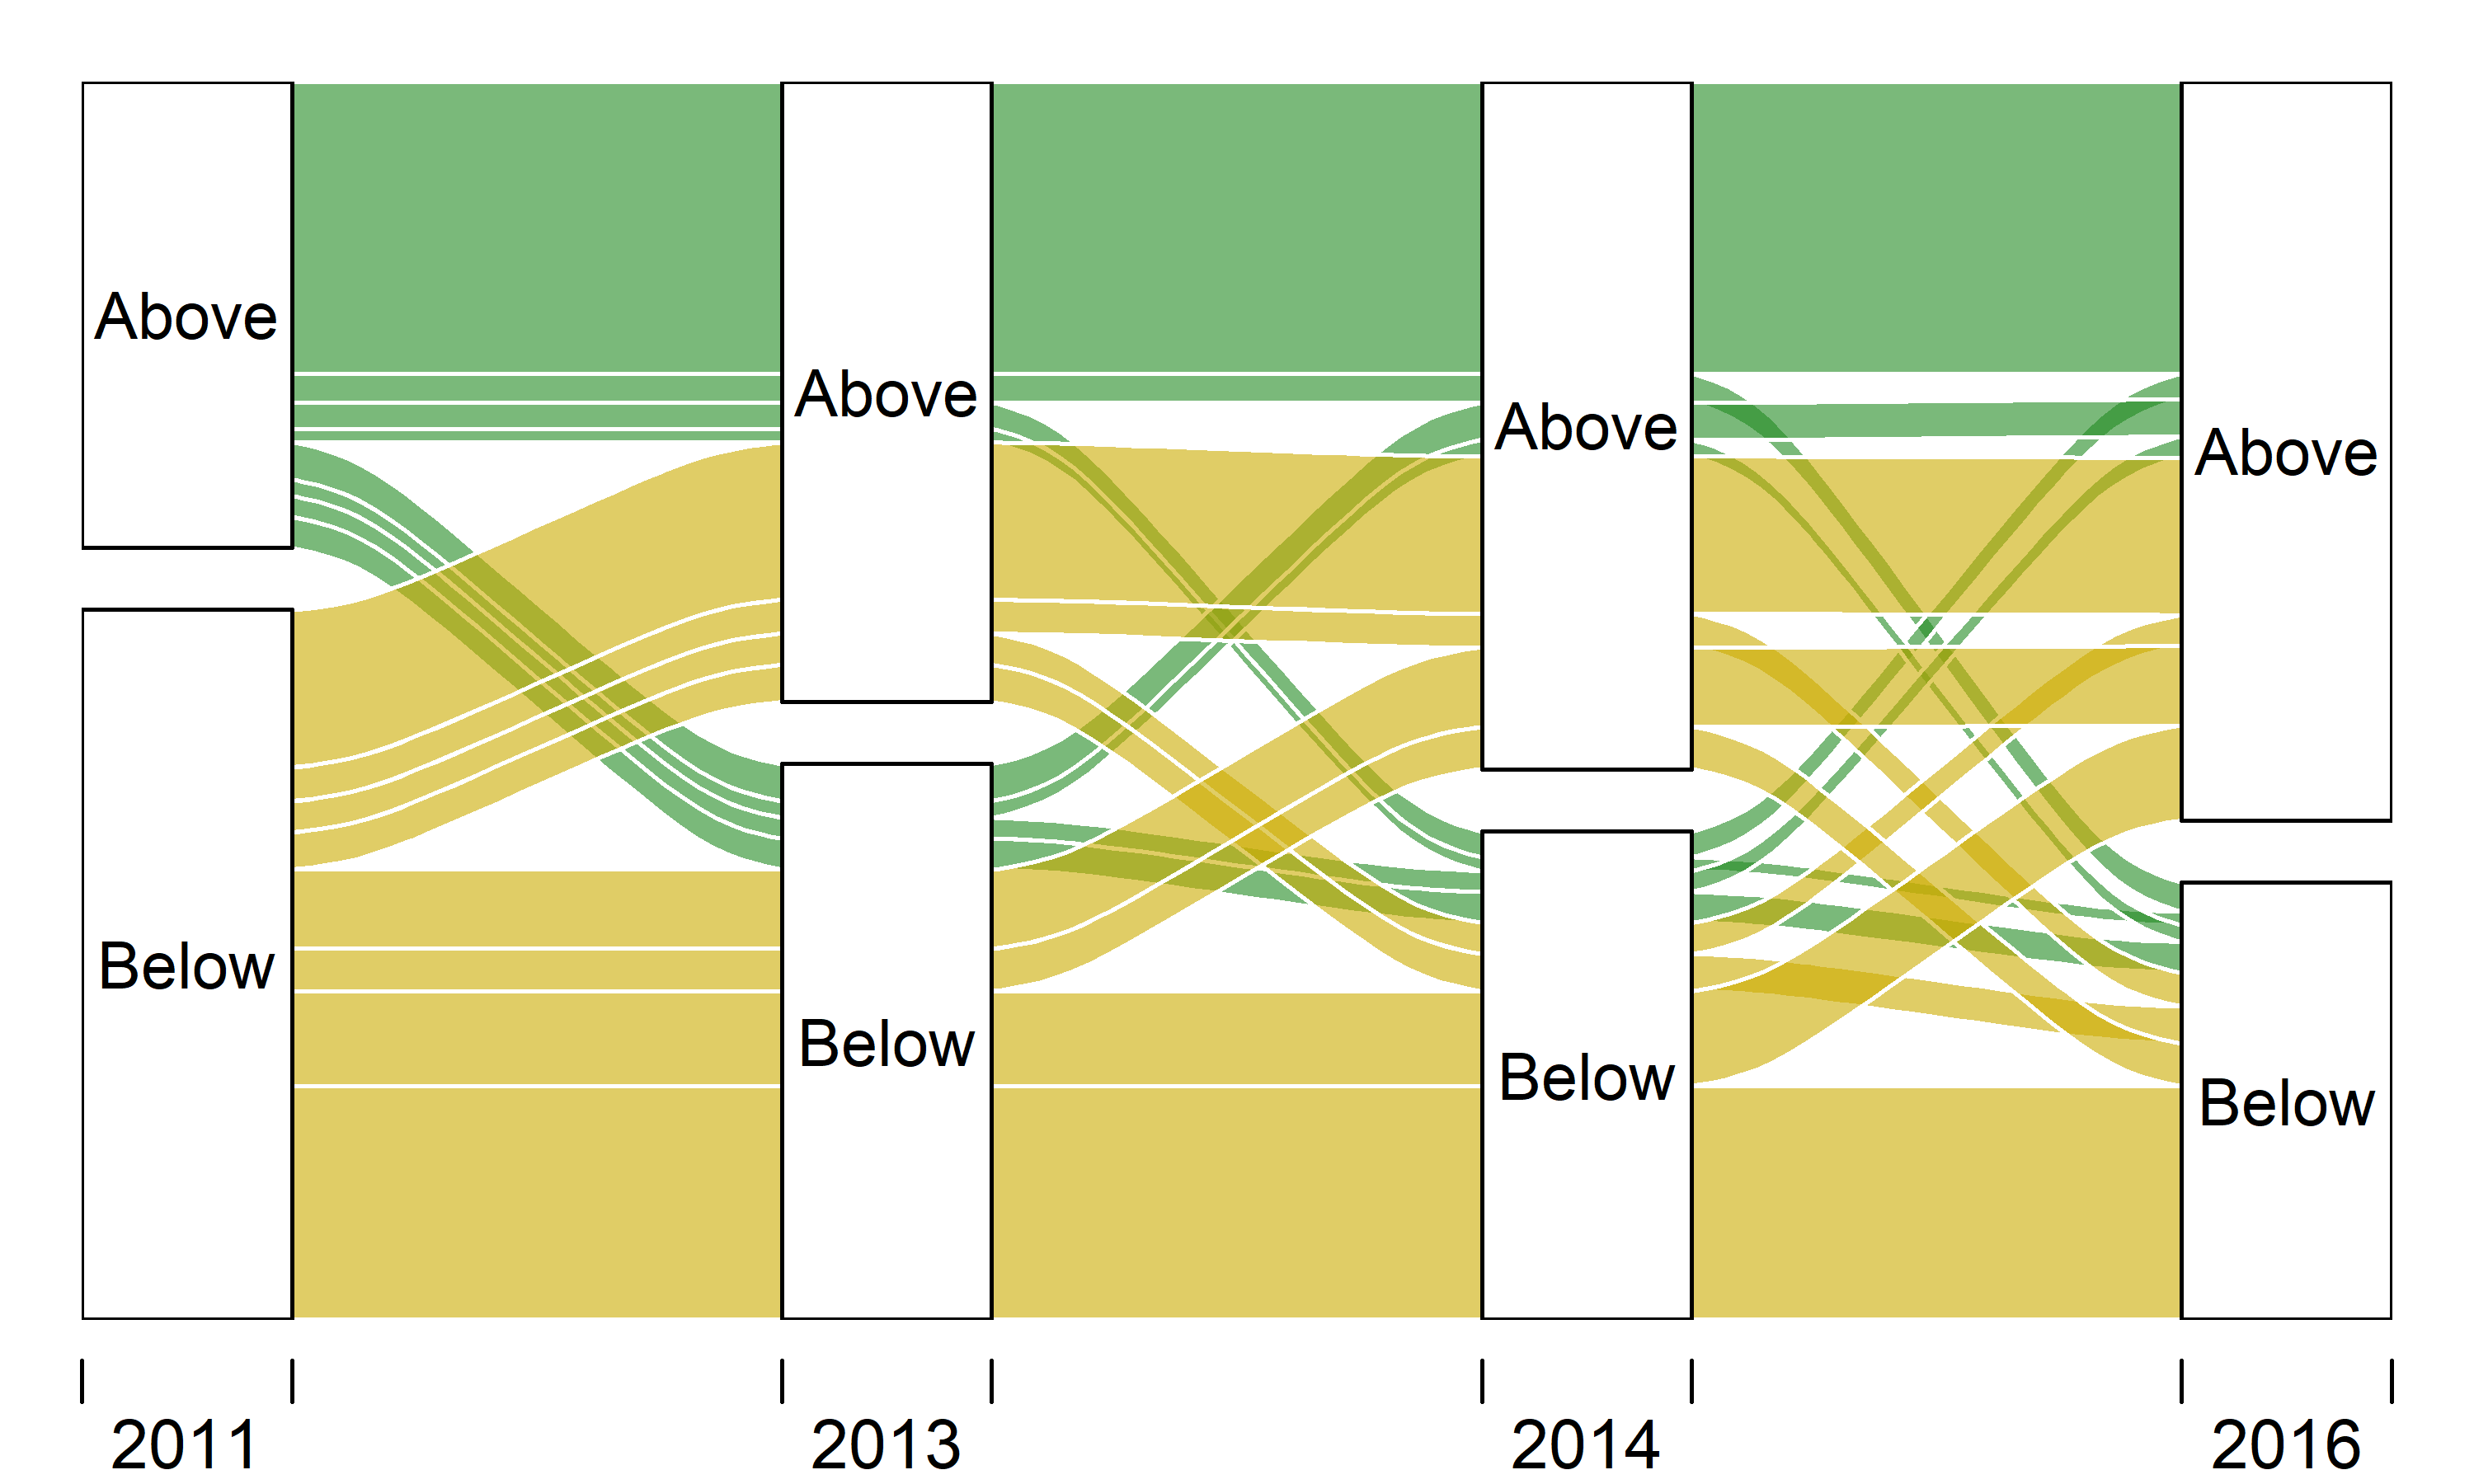
\includegraphics[width=1\textwidth]{Figures/bisp_poverty_alluvial.png}   
  \caption{Change in whether household is above or below BISP poverty threshold across OPM rounds}
  \label{fig:sub-first}
\end{subfigure}
\begin{subfigure}{.55\textwidth}
  \centering
  % include second image
  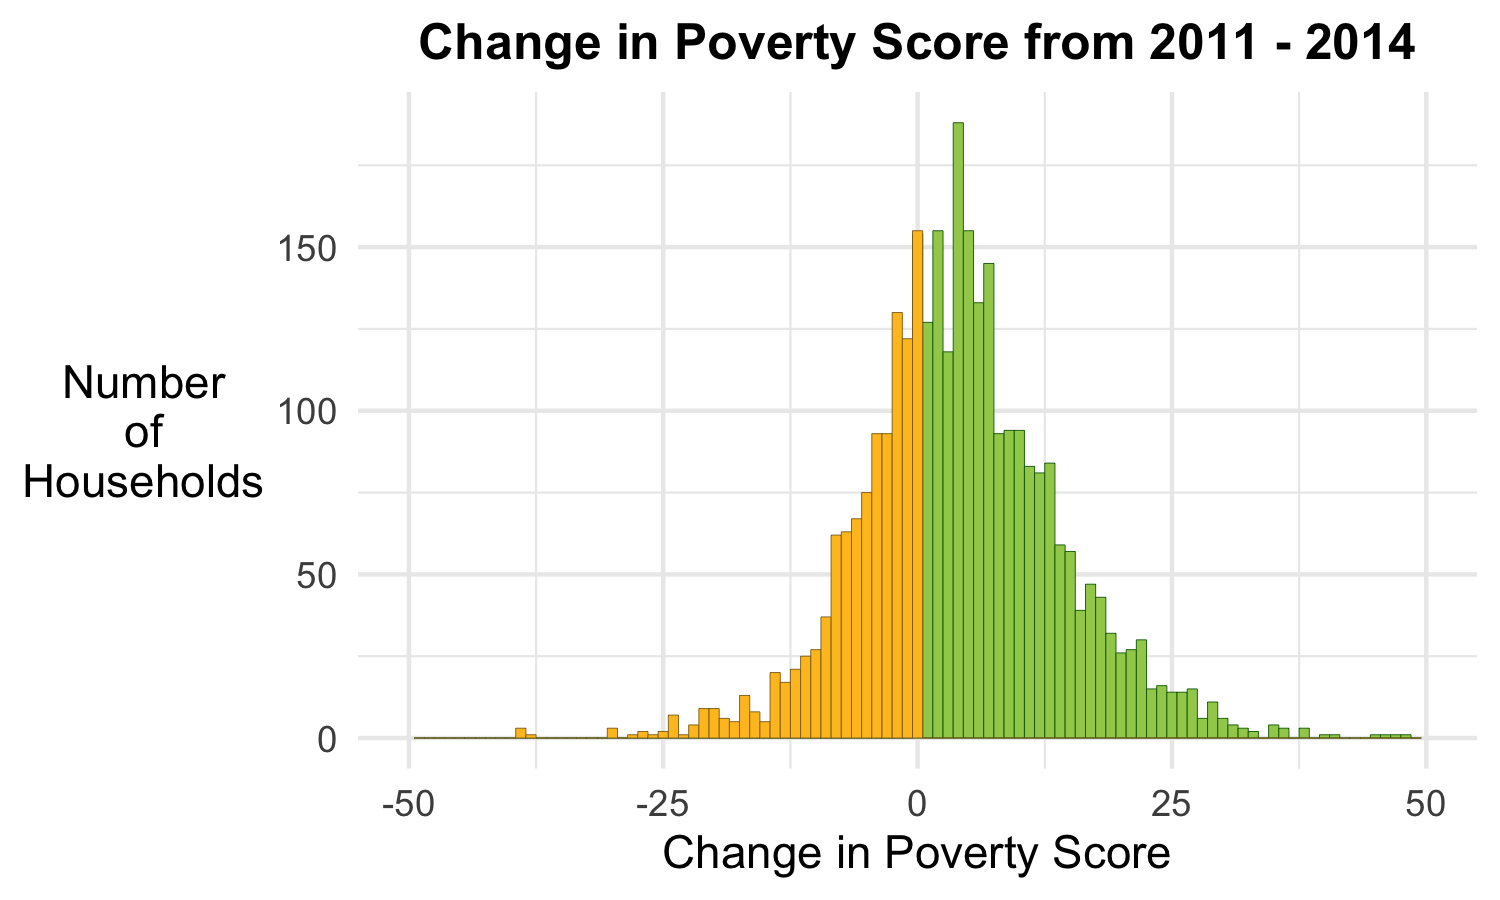
\includegraphics[trim=0 0 0 50mm,clip,width=1\textwidth]{Figures/pscore_changes_r13.png}   
  \caption{Change in poverty score from 2011-2014}
  \label{fig:sub-second}
\end{subfigure}
 \caption{Change in household poverty}     
\label{fig:pscore_change_hist}
\end{figure}




\newpage
\section{Data Sources Used for Poverty Estimation}

We rely on four sources of publicly available, nontraditional data sources to estimate poverty:
\begin{itemize}
\item {\bf Nighttime Lights:} We use nighttime lights data from the Visible Imaging Radiometer Suite (VIIRS) onboard the Suomi National Polar-orbiting Partnership satellite. VIIRS provides nighttime lights values for 750 meter pixels from April 2012 to the present. We extract monthly averages and create a number of metrics at the annual level, including average, minimum, maximum and standard deviation of nighttime lights across months in a year within areas 1, 2, 5 and 10km from each household. 
\item {\bf Daytime Imagery:} We use daytime imagery from landsat which is available from the 1980s to the present. Imagery is available at a 30 meter resolution roughly every two weeks. Landsat data contains seven bands, representing different reflectance along the electromagnetic spectrum (e.g., reflectance of visible light -- red, green and blue, and othe bands such as infrared). The individual bands themselves do not provide an intuitive meaning; however, combinations of bands provide an intutitive meaning. For example, combining red and infrared bands provides a measure of the amount of vegetation.
\item {\bf Facebook Useage:} We scrape data on daily and monthly active users on Facebook using Facebook's marketing API. The marketing API allows determining the number of facebook users by characteristics---for example, the number of male or female users, the number of users with a select educational background, or the type of phone (e.g., high end or cheap) used to access Facebook. 
\item {\bf Open Street Maps:} We integrate road data from Open Street Map, measuring the distance of households to the nearest road and nearest type of road --- for example, the nearest trunk road or residential road.
\end{itemize}

\autoref{tab:meanmedian_vars_by_poor} summarizes select variables from each data source by poverty level. Nighttime lights, a select indice from daytime imagery, daily active facebook users, and access to residential roads all appear higher among non-poor households compare to poor households. 

\begin{table}[H]
\caption{Summary Statistics of Nontraditional Data by Poverty Level}
\label{tab:meanmedian_vars_by_poor}
\centering
\begin{tabular}{l|cc|cc} 
\hline 
& \multicolumn{2}{c|}{Mean} & \multicolumn{2}{c}{Median} \\ 
Variable & Poor & Non-Poor & Poor & Non-Poor \\ 
\hline 
Nighttime Lights: Average & 1.86 & 3.54 & 0.5 & 0.67  \\ 
Daytime Imagery: Indice with Bands 2 and 5 & -0.07 & 0 & 0.02 & 0.1  \\ 
Facebook: All Daily Active Users & 16,596.67 & 40,968.09 & 0 & 498  \\ 
Facebook: Male Daily Active Users & 13,696.51 & 33,076.67 & 0 & 332  \\ 
Facebook: Female Daily Active Users & 3,000.17 & 7,858.67 & 0 & 0  \\ 
OSM: Kilometers to Residential Road & 4.75 & 4.27 & 2.63 & 1.41  \\ 
\hline 
\end{tabular} 
\flushleft \footnotesize The full sample includes all households while the sample with coordinates only includes households with a geocode.
\end{table}

\end{document}  




